% Informe del laboratorio 4: identificación, modelo analítico en espacio de estados y estructura física de la base
% Compilar desde esta carpeta: pdflatex informe_lab04.tex (dos veces)
\documentclass[a4paper,11pt]{article}
% Preámbulo común de los informes de laboratorio (II/2026). Se incluye desde laboratorios/labNN_*/
%   % Preámbulo común de los informes de laboratorio (II/2026). Se incluye desde laboratorios/labNN_*/
%   % Preámbulo común de los informes de laboratorio (II/2026). Se incluye desde laboratorios/labNN_*/
%   \input{../informe_comun}
\input{../../gemelo-digital/manual/estilo_manual}
\input{../../gemelo-digital/manual/tecnico/macros}
\graphicspath{{../../documentacion/planos_isa/pid/}{../../documentacion/planos_isa/electrico/}{../../documentacion/manuales_inversa/}
  {../../database/mockups/}{../../database/documentacion/}{../../database/modelo/}{../../database/interfaz/}
  {../../gemelo-digital/manual/img/}{../../modelo-3d/informe/figuras/}{../../modelo-3d/levantamiento/}{../../../../global/fotos-planta/}{../figuras/}}
\usepackage{pdflscape}
\lstset{showstringspaces=false}
% plano A3 en una página apaisada: \plano[página]{archivo}{leyenda}
\newcommand{\plano}[3][1]{\begin{landscape}\begin{figure}[p]\centering\includegraphics[page=#1, width=\linewidth, height=0.86\textwidth, keepaspectratio]{#2}\caption{#3}\end{figure}\end{landscape}}
\setlength{\headheight}{14pt}
\newcommand{\nlab}{}
\newcommand{\tlab}{}
\lhead{\small Brazo XK-JS1-1 · Informe del laboratorio \nlab}
\rhead{\small UMSA · II/2026}

% \portada{número}{título}{inicio}{entrega}{semanas}
\newcommand{\portada}[5]{%
\renewcommand{\nlab}{#1}%
\begin{titlepage}
\centering
\vspace*{0.6cm}
{\large Universidad Mayor de San Andrés · Facultad de Ingeniería\par}
{\large Carrera de Ingeniería Electrónica\par}
\vspace{0.8cm}
{\color{naranja!80!black}\rule{\linewidth}{1.5pt}\par}
\vspace{0.3cm}
{\Large Informe del Laboratorio Integrado Nº #1\par}
\vspace{0.2cm}
{\huge\bfseries #2\par}
\vspace{0.3cm}
{\color{naranja!80!black}\rule{\linewidth}{1.5pt}\par}
\vspace{0.8cm}
{\large Planta: brazo robótico XK-JS1-1 de 4 grados de libertad\par}
\vspace{0.3cm}
{\large ETN-902 Sistemas de Control II · ETN-1034 Aplicación de Técnicas de Control · ETN-1000 Bases de Datos\par}
\vspace{1cm}
\begin{tabular}{rl}
\textbf{Docente:} & Ing. Jorge Antonio Nava Amador\\
\textbf{Auxiliares:} & Limber Ajnota · Fabián Plata · Franz Choque\\
\textbf{Inicio de trabajo:} & #3\\
\textbf{Entrega:} & #4 (#5)\\
\end{tabular}
\vspace{1cm}

\begin{tabular}{ll}
\multicolumn{2}{l}{\textbf{Escuadra del brazo de 4 GDL}}\\[2pt]
Control (ETN-902 / ETN-1034): & Gabriel Andres Gomez Calla\\
 & Jose Lenin Mamani Choque\\
 & Miguel Alejandro Lima Huarachi\\
 & Román Abner Machicado Arequipa\\[2pt]
Cómputo (ETN-1000): & Miguel Alejandro Lima Huarachi\\
 & Marco Eduardo Chura Rondo\\
\end{tabular}
\vfill
{\small Repositorio: \url{https://github.com/GabAndGom/Brazo-de-4-grados-de-libertad}\par}
{\small La Paz, Bolivia · gestión II/2026\par}
\end{titlepage}
}

% Tabla de entregables (Definition of Done): \begin{dod} ... \end{dod}, filas: entregable & estado & evidencia\\
\newenvironment{dod}{\begin{center}\small\begin{longtable}{>{\raggedright}p{5.2cm} >{\raggedright}p{1.8cm} >{\raggedright\arraybackslash}p{7.6cm}}
\toprule \textbf{Entregable} & \textbf{Estado} & \textbf{Evidencia / observación}\\ \midrule \endhead}
{\bottomrule\end{longtable}\end{center}}

\input{../../gemelo-digital/manual/estilo_manual}
% Macros del manual técnico: ladder, estados, código y rutas de imágenes
\usetikzlibrary{shapes.multipart}
\graphicspath{{../img/}{../../../../../global/fotos-planta/}{../../../modelo-3d/informe/figuras/}{../../../modelo-3d/levantamiento/}{../../../database/modelo/}{../../../documentacion/manuales_inversa/}{../../../documentacion/planos_isa/electrico/}{../../../database/interfaz/}}

\lstdefinestyle{py}{language=Python, keywordstyle=\color{azulg}\bfseries, commentstyle=\color{grisos}\itshape,
  stringstyle=\color{verde}, basicstyle=\ttfamily\scriptsize, numbers=left, numberstyle=\tiny\color{grisos}}
\lstdefinestyle{js}{language=Java, morekeywords={const,let,function,async,await,return,for,of,if,else}, keywordstyle=\color{azulg}\bfseries,
  commentstyle=\color{grisos}\itshape, stringstyle=\color{verde}, basicstyle=\ttfamily\scriptsize, numbers=left, numberstyle=\tiny\color{grisos}}
\lstdefinestyle{awl}{basicstyle=\ttfamily\tiny, commentstyle=\color{grisos}\itshape, morecomment=[l]{//},
  keywordstyle=\color{azulg}\bfseries, morekeywords={LD,LDN,A,AN,O,ON,EU,ED,S,R,MOVB,MOVW,MOVD,PLS,TON,CALL,CRET,LPS,LRD,LPP,ALD,OLD,FILL,LDW,LDB,LDD,AW,AD,AB,OW,OD},
  numbers=left, numberstyle=\tiny\color{grisos}, frame=single, backgroundcolor=\color{gris}}
\lstdefinestyle{sql}{language=SQL, keywordstyle=\color{azulg}\bfseries, commentstyle=\color{grisos}\itshape,
  stringstyle=\color{verde}, basicstyle=\ttfamily\tiny, numbers=left, numberstyle=\tiny\color{grisos},
  morekeywords={REFERENCES,SERIAL,SMALLSERIAL,BIGSERIAL,TIMESTAMPTZ,BOOLEAN,INET,RETURNS,TRIGGER,LANGUAGE,DECLARE,RAISE,EXCEPTION,VIEW,INDEX}}

\tikzset{
  ld/.style={line width=0.7pt},
  pics/na/.style={code={\fill[white](-0.12,-0.26) rectangle (0.12,0.26);
     \draw[thick](-0.1,-0.24)--(-0.1,0.24)(0.1,-0.24)--(0.1,0.24);
     \node[font=\scriptsize\ttfamily, above] at (0,0.22){#1};}},
  pics/nc/.style={code={\fill[white](-0.12,-0.26) rectangle (0.12,0.26);
     \draw[thick](-0.1,-0.24)--(-0.1,0.24)(0.1,-0.24)--(0.1,0.24);\draw(-0.17,-0.24)--(0.17,0.24);
     \node[font=\scriptsize\ttfamily, above] at (0,0.22){#1};}},
  pics/pf/.style={code={\fill[white](-0.12,-0.26) rectangle (0.12,0.26);
     \draw[thick](-0.1,-0.24)--(-0.1,0.24)(0.1,-0.24)--(0.1,0.24);
     \node[font=\tiny\bfseries] at (0,0){P};}},
  pics/cmp/.style n args={3}{code={\fill[white](-0.12,-0.26) rectangle (0.12,0.26);
     \draw[thick](-0.1,-0.24)--(-0.1,0.24)(0.1,-0.24)--(0.1,0.24);
     \node[font=\tiny\ttfamily] at (0,0){#2};
     \node[font=\scriptsize\ttfamily, above] at (0,0.22){#1};
     \node[font=\scriptsize\ttfamily, below] at (0,-0.22){#3};}},
  pics/bob/.style n args={3}{code={\fill[white](-0.2,-0.26) rectangle (0.2,0.26);
     \draw[thick](-0.05,0.24) arc (110:250:0.255);\draw[thick](0.05,0.24) arc (70:-70:0.255);
     \node[font=\tiny\bfseries] at (0,0){#2};
     \node[font=\scriptsize\ttfamily, above] at (0,0.22){#1};
     \node[font=\scriptsize\ttfamily, below] at (0,-0.22){#3};}},
  fb/.style={draw, fill=white, font=\scriptsize\ttfamily, align=left, inner sep=3pt, anchor=west},
  barra/.style={line width=2pt},
  estado/.style={draw, rounded corners=3pt, fill=white, align=center, font=\scriptsize, minimum width=22mm, minimum height=10mm, inner sep=3pt},
  estadon/.style={estado, fill=naranja!14, draw=naranja!70!black},
  trans/.style={font=\scriptsize, align=center, fill=white, inner sep=1pt},
  lugar/.style={circle, draw, thick, minimum size=7mm, fill=white},
  transicion/.style={rectangle, fill=black, minimum width=1.6mm, minimum height=7mm, inner sep=0},
  tabla/.style={rectangle split, rectangle split parts=2, draw, fill=white, font=\tiny\ttfamily, align=left, inner sep=2pt, rounded corners=1pt, text width=33mm},
}
\newcommand{\pendiente}[1]{\par\smallskip\noindent\colorbox{naranja!12}{\parbox{\dimexpr\linewidth-2\fboxsep}{\textbf{\color{naranja!80!black}Pendiente.} #1}}\par\smallskip}
\newcommand{\cumple}{\textcolor{verde}{\textbf{cumplido}}}
\newcommand{\parcial}{\textcolor{naranja}{\textbf{parcial}}}
\newcommand{\falta}{\textcolor{rojo}{\textbf{pendiente}}}

\graphicspath{{../../documentacion/planos_isa/pid/}{../../documentacion/planos_isa/electrico/}{../../documentacion/manuales_inversa/}
  {../../database/mockups/}{../../database/documentacion/}{../../database/modelo/}{../../database/interfaz/}
  {../../gemelo-digital/manual/img/}{../../modelo-3d/informe/figuras/}{../../modelo-3d/levantamiento/}{../../../../global/fotos-planta/}{../figuras/}}
\usepackage{pdflscape}
\lstset{showstringspaces=false}
% plano A3 en una página apaisada: \plano[página]{archivo}{leyenda}
\newcommand{\plano}[3][1]{\begin{landscape}\begin{figure}[p]\centering\includegraphics[page=#1, width=\linewidth, height=0.86\textwidth, keepaspectratio]{#2}\caption{#3}\end{figure}\end{landscape}}
\setlength{\headheight}{14pt}
\newcommand{\nlab}{}
\newcommand{\tlab}{}
\lhead{\small Brazo XK-JS1-1 · Informe del laboratorio \nlab}
\rhead{\small UMSA · II/2026}

% \portada{número}{título}{inicio}{entrega}{semanas}
\newcommand{\portada}[5]{%
\renewcommand{\nlab}{#1}%
\begin{titlepage}
\centering
\vspace*{0.6cm}
{\large Universidad Mayor de San Andrés · Facultad de Ingeniería\par}
{\large Carrera de Ingeniería Electrónica\par}
\vspace{0.8cm}
{\color{naranja!80!black}\rule{\linewidth}{1.5pt}\par}
\vspace{0.3cm}
{\Large Informe del Laboratorio Integrado Nº #1\par}
\vspace{0.2cm}
{\huge\bfseries #2\par}
\vspace{0.3cm}
{\color{naranja!80!black}\rule{\linewidth}{1.5pt}\par}
\vspace{0.8cm}
{\large Planta: brazo robótico XK-JS1-1 de 4 grados de libertad\par}
\vspace{0.3cm}
{\large ETN-902 Sistemas de Control II · ETN-1034 Aplicación de Técnicas de Control · ETN-1000 Bases de Datos\par}
\vspace{1cm}
\begin{tabular}{rl}
\textbf{Docente:} & Ing. Jorge Antonio Nava Amador\\
\textbf{Auxiliares:} & Limber Ajnota · Fabián Plata · Franz Choque\\
\textbf{Inicio de trabajo:} & #3\\
\textbf{Entrega:} & #4 (#5)\\
\end{tabular}
\vspace{1cm}

\begin{tabular}{ll}
\multicolumn{2}{l}{\textbf{Escuadra del brazo de 4 GDL}}\\[2pt]
Control (ETN-902 / ETN-1034): & Gabriel Andres Gomez Calla\\
 & Jose Lenin Mamani Choque\\
 & Miguel Alejandro Lima Huarachi\\
 & Román Abner Machicado Arequipa\\[2pt]
Cómputo (ETN-1000): & Miguel Alejandro Lima Huarachi\\
 & Marco Eduardo Chura Rondo\\
\end{tabular}
\vfill
{\small Repositorio: \url{https://github.com/GabAndGom/Brazo-de-4-grados-de-libertad}\par}
{\small La Paz, Bolivia · gestión II/2026\par}
\end{titlepage}
}

% Tabla de entregables (Definition of Done): \begin{dod} ... \end{dod}, filas: entregable & estado & evidencia\\
\newenvironment{dod}{\begin{center}\small\begin{longtable}{>{\raggedright}p{5.2cm} >{\raggedright}p{1.8cm} >{\raggedright\arraybackslash}p{7.6cm}}
\toprule \textbf{Entregable} & \textbf{Estado} & \textbf{Evidencia / observación}\\ \midrule \endhead}
{\bottomrule\end{longtable}\end{center}}

\input{../../gemelo-digital/manual/estilo_manual}
% Macros del manual técnico: ladder, estados, código y rutas de imágenes
\usetikzlibrary{shapes.multipart}
\graphicspath{{../img/}{../../../../../global/fotos-planta/}{../../../modelo-3d/informe/figuras/}{../../../modelo-3d/levantamiento/}{../../../database/modelo/}{../../../documentacion/manuales_inversa/}{../../../documentacion/planos_isa/electrico/}{../../../database/interfaz/}}

\lstdefinestyle{py}{language=Python, keywordstyle=\color{azulg}\bfseries, commentstyle=\color{grisos}\itshape,
  stringstyle=\color{verde}, basicstyle=\ttfamily\scriptsize, numbers=left, numberstyle=\tiny\color{grisos}}
\lstdefinestyle{js}{language=Java, morekeywords={const,let,function,async,await,return,for,of,if,else}, keywordstyle=\color{azulg}\bfseries,
  commentstyle=\color{grisos}\itshape, stringstyle=\color{verde}, basicstyle=\ttfamily\scriptsize, numbers=left, numberstyle=\tiny\color{grisos}}
\lstdefinestyle{awl}{basicstyle=\ttfamily\tiny, commentstyle=\color{grisos}\itshape, morecomment=[l]{//},
  keywordstyle=\color{azulg}\bfseries, morekeywords={LD,LDN,A,AN,O,ON,EU,ED,S,R,MOVB,MOVW,MOVD,PLS,TON,CALL,CRET,LPS,LRD,LPP,ALD,OLD,FILL,LDW,LDB,LDD,AW,AD,AB,OW,OD},
  numbers=left, numberstyle=\tiny\color{grisos}, frame=single, backgroundcolor=\color{gris}}
\lstdefinestyle{sql}{language=SQL, keywordstyle=\color{azulg}\bfseries, commentstyle=\color{grisos}\itshape,
  stringstyle=\color{verde}, basicstyle=\ttfamily\tiny, numbers=left, numberstyle=\tiny\color{grisos},
  morekeywords={REFERENCES,SERIAL,SMALLSERIAL,BIGSERIAL,TIMESTAMPTZ,BOOLEAN,INET,RETURNS,TRIGGER,LANGUAGE,DECLARE,RAISE,EXCEPTION,VIEW,INDEX}}

\tikzset{
  ld/.style={line width=0.7pt},
  pics/na/.style={code={\fill[white](-0.12,-0.26) rectangle (0.12,0.26);
     \draw[thick](-0.1,-0.24)--(-0.1,0.24)(0.1,-0.24)--(0.1,0.24);
     \node[font=\scriptsize\ttfamily, above] at (0,0.22){#1};}},
  pics/nc/.style={code={\fill[white](-0.12,-0.26) rectangle (0.12,0.26);
     \draw[thick](-0.1,-0.24)--(-0.1,0.24)(0.1,-0.24)--(0.1,0.24);\draw(-0.17,-0.24)--(0.17,0.24);
     \node[font=\scriptsize\ttfamily, above] at (0,0.22){#1};}},
  pics/pf/.style={code={\fill[white](-0.12,-0.26) rectangle (0.12,0.26);
     \draw[thick](-0.1,-0.24)--(-0.1,0.24)(0.1,-0.24)--(0.1,0.24);
     \node[font=\tiny\bfseries] at (0,0){P};}},
  pics/cmp/.style n args={3}{code={\fill[white](-0.12,-0.26) rectangle (0.12,0.26);
     \draw[thick](-0.1,-0.24)--(-0.1,0.24)(0.1,-0.24)--(0.1,0.24);
     \node[font=\tiny\ttfamily] at (0,0){#2};
     \node[font=\scriptsize\ttfamily, above] at (0,0.22){#1};
     \node[font=\scriptsize\ttfamily, below] at (0,-0.22){#3};}},
  pics/bob/.style n args={3}{code={\fill[white](-0.2,-0.26) rectangle (0.2,0.26);
     \draw[thick](-0.05,0.24) arc (110:250:0.255);\draw[thick](0.05,0.24) arc (70:-70:0.255);
     \node[font=\tiny\bfseries] at (0,0){#2};
     \node[font=\scriptsize\ttfamily, above] at (0,0.22){#1};
     \node[font=\scriptsize\ttfamily, below] at (0,-0.22){#3};}},
  fb/.style={draw, fill=white, font=\scriptsize\ttfamily, align=left, inner sep=3pt, anchor=west},
  barra/.style={line width=2pt},
  estado/.style={draw, rounded corners=3pt, fill=white, align=center, font=\scriptsize, minimum width=22mm, minimum height=10mm, inner sep=3pt},
  estadon/.style={estado, fill=naranja!14, draw=naranja!70!black},
  trans/.style={font=\scriptsize, align=center, fill=white, inner sep=1pt},
  lugar/.style={circle, draw, thick, minimum size=7mm, fill=white},
  transicion/.style={rectangle, fill=black, minimum width=1.6mm, minimum height=7mm, inner sep=0},
  tabla/.style={rectangle split, rectangle split parts=2, draw, fill=white, font=\tiny\ttfamily, align=left, inner sep=2pt, rounded corners=1pt, text width=33mm},
}
\newcommand{\pendiente}[1]{\par\smallskip\noindent\colorbox{naranja!12}{\parbox{\dimexpr\linewidth-2\fboxsep}{\textbf{\color{naranja!80!black}Pendiente.} #1}}\par\smallskip}
\newcommand{\cumple}{\textcolor{verde}{\textbf{cumplido}}}
\newcommand{\parcial}{\textcolor{naranja}{\textbf{parcial}}}
\newcommand{\falta}{\textcolor{rojo}{\textbf{pendiente}}}

\graphicspath{{../../documentacion/planos_isa/pid/}{../../documentacion/planos_isa/electrico/}{../../documentacion/manuales_inversa/}
  {../../database/mockups/}{../../database/documentacion/}{../../database/modelo/}{../../database/interfaz/}
  {../../gemelo-digital/manual/img/}{../../modelo-3d/informe/figuras/}{../../modelo-3d/levantamiento/}{../../../../global/fotos-planta/}{../figuras/}}
\usepackage{pdflscape}
\lstset{showstringspaces=false}
% plano A3 en una página apaisada: \plano[página]{archivo}{leyenda}
\newcommand{\plano}[3][1]{\begin{landscape}\begin{figure}[p]\centering\includegraphics[page=#1, width=\linewidth, height=0.86\textwidth, keepaspectratio]{#2}\caption{#3}\end{figure}\end{landscape}}
\setlength{\headheight}{14pt}
\newcommand{\nlab}{}
\newcommand{\tlab}{}
\lhead{\small Brazo XK-JS1-1 · Informe del laboratorio \nlab}
\rhead{\small UMSA · II/2026}

% \portada{número}{título}{inicio}{entrega}{semanas}
\newcommand{\portada}[5]{%
\renewcommand{\nlab}{#1}%
\begin{titlepage}
\centering
\vspace*{0.6cm}
{\large Universidad Mayor de San Andrés · Facultad de Ingeniería\par}
{\large Carrera de Ingeniería Electrónica\par}
\vspace{0.8cm}
{\color{naranja!80!black}\rule{\linewidth}{1.5pt}\par}
\vspace{0.3cm}
{\Large Informe del Laboratorio Integrado Nº #1\par}
\vspace{0.2cm}
{\huge\bfseries #2\par}
\vspace{0.3cm}
{\color{naranja!80!black}\rule{\linewidth}{1.5pt}\par}
\vspace{0.8cm}
{\large Planta: brazo robótico XK-JS1-1 de 4 grados de libertad\par}
\vspace{0.3cm}
{\large ETN-902 Sistemas de Control II · ETN-1034 Aplicación de Técnicas de Control · ETN-1000 Bases de Datos\par}
\vspace{1cm}
\begin{tabular}{rl}
\textbf{Docente:} & Ing. Jorge Antonio Nava Amador\\
\textbf{Auxiliares:} & Limber Ajnota · Fabián Plata · Franz Choque\\
\textbf{Inicio de trabajo:} & #3\\
\textbf{Entrega:} & #4 (#5)\\
\end{tabular}
\vspace{1cm}

\begin{tabular}{ll}
\multicolumn{2}{l}{\textbf{Escuadra del brazo de 4 GDL}}\\[2pt]
Control (ETN-902 / ETN-1034): & Gabriel Andres Gomez Calla\\
 & Jose Lenin Mamani Choque\\
 & Miguel Alejandro Lima Huarachi\\
 & Román Abner Machicado Arequipa\\[2pt]
Cómputo (ETN-1000): & Miguel Alejandro Lima Huarachi\\
 & Marco Eduardo Chura Rondo\\
\end{tabular}
\vfill
{\small Repositorio: \url{https://github.com/GabAndGom/Brazo-de-4-grados-de-libertad}\par}
{\small La Paz, Bolivia · gestión II/2026\par}
\end{titlepage}
}

% Tabla de entregables (Definition of Done): \begin{dod} ... \end{dod}, filas: entregable & estado & evidencia\\
\newenvironment{dod}{\begin{center}\small\begin{longtable}{>{\raggedright}p{5.2cm} >{\raggedright}p{1.8cm} >{\raggedright\arraybackslash}p{7.6cm}}
\toprule \textbf{Entregable} & \textbf{Estado} & \textbf{Evidencia / observación}\\ \midrule \endhead}
{\bottomrule\end{longtable}\end{center}}


\begin{document}
\portada{4}{Identificación de la planta, modelo en espacio de estados y estructura física de la base de datos}{martes 15 de septiembre de 2026}{martes 29 de septiembre de 2026}{semanas 7 y 8}

\tableofcontents
\newpage

\section{Objetivos}
\begin{itemize}
\item \textbf{ETN-902}: aproximar la función de transferencia de la planta por pruebas de estímulo-respuesta (caja negra).
\item \textbf{ETN-1034}: formular las ecuaciones del sistema y representarlo en espacio de estados, $\dot{x} = Ax + Bu$.
\item \textbf{ETN-1000}: llevar el modelo lógico a PostgreSQL con un script DDL, tipos de datos, PK, FK, NOT NULL e integridad referencial.
\end{itemize}

\section{Alcance y seguridad}
La guía prohíbe excitar los actuadores con señales desproporcionadas. En el brazo, la «señal escalón» es un cambio de frecuencia del tren de pulsos dentro del rango probado sin pérdida de pasos: 500 a 5000~Hz en los carros y 2,5~kHz en la base (manual técnico, capítulo 4). Los datos deben exportarse en texto (CSV).

\section{ETN-902: identificación por caja negra}
\subsection{Qué se puede medir en esta planta}
La identificación por curva de reacción necesita medir la salida $y(t)$. En el brazo no hay transmisor de posición: la posición que muestra el gemelo se \emph{calcula} contando los pulsos enviados, así que comparar esa posición con la entrada no identifica nada (es la entrada integrada). Las únicas mediciones independientes son los instantes en que se activan los finales de carrera (I0.1--I0.4) y el sensor inductivo (I0.0).

\subsection{Prueba automatizada: \codigo{prueba\_escalon.py}}
La prueba se automatizó sobre la app del gemelo (actualización del 18/11/2026). El script toma el mando, hace homing si falta, lleva el eje a 0~mm y aplica un escalón de frecuencia de 0 a $f$ hacia el otro extremo (170~mm), registrando cada lectura del PLC en un CSV hasta que el eje se detiene:
\begin{lstlisting}[language=bash]
python3 prueba_escalon.py --eje X --frecuencias 1000 2000 3000 4000   # con la app abierta
python3 prueba_escalon.py --analizar "datos/escalon_X_*.csv"
\end{lstlisting}
Columnas del CSV: tiempo desde la orden, frecuencia ordenada, posición y pulsos informados por el PLC, bandera de movimiento, finales de carrera, error del PLC y edad de la lectura.

\paragraph{Qué se mide de verdad.} El PLC suma los pulsos del tramo al terminarlo: la posición intermedia que muestra la app es una interpolación con la frecuencia ordenada, no una medición. Por eso el análisis usa solo lo que informa el PLC: el instante en que empieza a moverse ($t_d$, tiempo muerto: latencia PPI más el ciclo del PLC) y el instante en que termina (velocidad media y ganancia $K = v/f$). La constante $\tau$ del conjunto motor--carro no se puede medir sin un sensor continuo.

\subsection{Resultados con el PLC simulado}
\aviso{Los datos de esta sección son del \textbf{PLC simulado} de la app (archivos \codigo{datos/escalon\_X\_*\_SIMULADO\_*.csv}): validan el procedimiento y el análisis, no la planta. La corrida en la planta queda pendiente para la próxima sesión de laboratorio, con el mismo comando y la app en «Operación local».}
\begin{center}\small
\begin{tabular}{c c c c c c}
\toprule
$f$ [Hz] & $t_d$ [s] & duración [s] & $d$ [mm] & $v$ [mm/s] & $K/K_{nom}$\\
\midrule
1000 & 0,027 & 34,008 & 170 & 5,00 & 1,000\\
2000 & 0,050 & 17,012 & 170 & 9,99 & 0,999\\
3000 & 0,027 & 11,342 & 170 & 14,99 & 0,999\\
4000 & 0,027 & 8,514 & 170 & 19,97 & 0,998\\
\bottomrule
\end{tabular}
\end{center}
\begin{figure}[H]
\centering
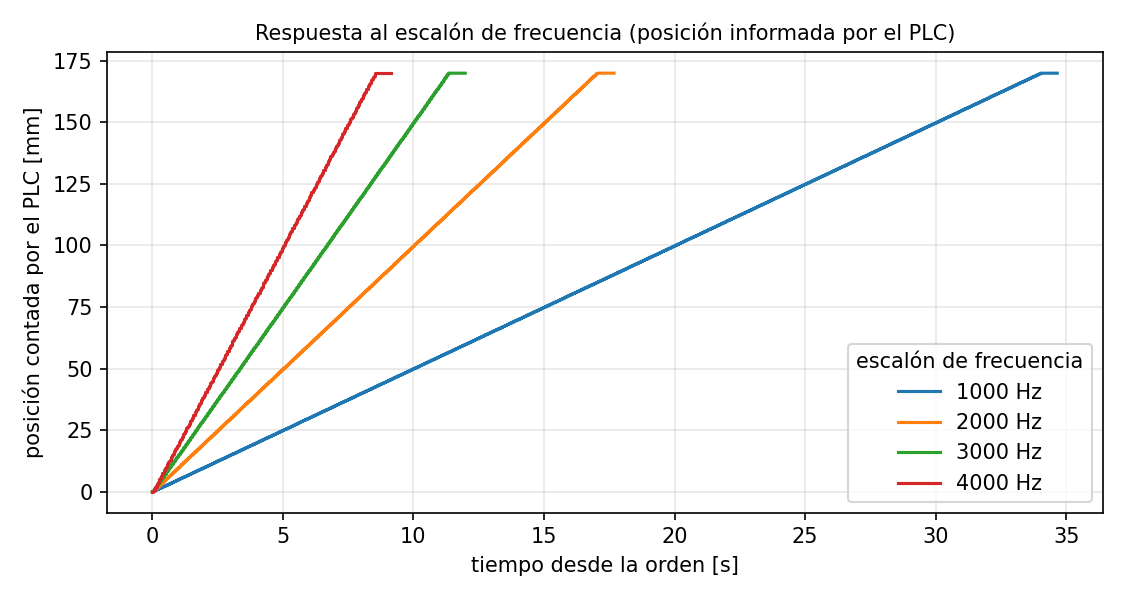
\includegraphics[width=0.75\linewidth]{datos/escalon_respuesta.png}
\caption{Respuesta al escalón de frecuencia (PLC simulado): posición informada por el PLC.}
\end{figure}
Modelo identificado por eje: $S(s)/F(s) = K e^{-t_d s}/s$, un integrador con tiempo muerto ($K_{nom} = 0{,}005$~mm/(Hz$\cdot$s)). Con la planta real se espera un $t_d$ mayor (cada lectura PPI tarda $\approx$155~ms) y, si el motor pierde pasos, una diferencia entre la posición contada y la real que solo revela una medición independiente (finales de carrera o calibre, laboratorio 5). Con un encoder o una regla lineal la curva completa permitiría aplicar los métodos de Smith o Sundaresan.

\section{ETN-1034: modelo analítico en espacio de estados}
\subsection{Leyes físicas}
Cada eje lo mueve un motor paso a paso con driver configurado a 1000 pulsos por vuelta. Mientras el par del motor alcanza (no se pierden pasos), cada pulso avanza el eje un ángulo fijo; la dinámica mecánica (inercia, fricción) solo decide \emph{si} el motor sigue al tren, no \emph{cuánto} avanza. Entonces:
\[
\dot\theta = \frac{f_0}{k_\theta}, \qquad \dot s_X = \kappa_1\frac{f_1}{k_{XY}}, \qquad \dot s_Y = \kappa_2\frac{f_1}{k_{XY}},
\]
con $k_\theta = 190{,}3$~pulsos/° $= 10\,903$~pulsos/rad (medido), $k_{XY} = 200$~pulsos/mm (1000~pulsos/vuelta con husillo de 5~mm, SUPUESTO), $f_0$ y $f_1$ las frecuencias de los trenes PTO0 y PTO1 (con signo según la salida de dirección) y $\kappa_1, \kappa_2 \in \{0, 1\}$ el estado de los relés K1 y K2.

\subsection{Forma matricial}
\[
\mathbf{x} = \begin{bmatrix}\theta\\ s_X\\ s_Y\end{bmatrix},\quad
\mathbf{u} = \begin{bmatrix}f_0\\ f_1\end{bmatrix},\quad
\dot{\mathbf{x}} = \underbrace{\begin{bmatrix}0&0&0\\0&0&0\\0&0&0\end{bmatrix}}_{A}\mathbf{x} +
\underbrace{\begin{bmatrix}9{,}17\cdot10^{-5} & 0\\ 0 & 0{,}005\,\kappa_1\\ 0 & 0{,}005\,\kappa_2\end{bmatrix}}_{B(\kappa)}\mathbf{u}
\]
\begin{itemize}
\item $x_1 = \theta$: ángulo de la base [rad]; $x_2 = s_X$: posición del carro X (alcance) [mm]; $x_3 = s_Y$: posición del carro Y (altura) [mm].
\item $A = 0$: sin entrada, ningún eje se mueve (el motor paso a paso retiene la posición).
\item $B$ depende de los relés: es un \textbf{sistema conmutado}. La salida Q0.1 es una sola, por eso X e Y comparten la misma frecuencia.
\end{itemize}

\subsection{Ecuación de salida}
Lo que interesa es la posición de la garra $\mathbf{p} = (X, Y, Z)$. La cinemática directa es no lineal; alrededor de un punto de operación $q_0$ se linealiza con el jacobiano (manual técnico, capítulo 8): $\Delta\mathbf{p} = J(q_0)\,\Delta\mathbf{x}$. En el centro del espacio de trabajo $(0°, 85, 85)$, con las cotas del modelo de Inventor del equipo:
\[
C = J(q_0) = \begin{bmatrix} 0 & 1 & -0{,}412\\ 578{,}8 & 0 & 0\\ 0 & 0 & 2{,}760\end{bmatrix}, \qquad D = 0 .
\]

\subsection{Función de transferencia}
Cada eje es un integrador puro:
\[
\frac{\Theta(s)}{F_0(s)} = \frac{9{,}17\cdot10^{-5}}{s}~\frac{\text{rad}}{\text{Hz}}, \qquad \frac{S_X(s)}{F_1(s)} = \frac{0{,}005}{s}~\frac{\text{mm}}{\text{Hz}} .
\]
No tiene la forma $Ke^{-t_ds}/(\tau s + 1)$ de la guía porque no hay polo estable: la dinámica de primer orden del conjunto motor--carro (si existe, de milisegundos) solo se podría ver con un sensor continuo.

\nota{\textbf{Modelo dinámico completo.} Si se quiere incluir la mecánica, cada eje agrega dos estados (ángulo y velocidad del rotor): $J_m\ddot\phi = T_m(\phi, \phi_{ref}) - b\dot\phi - T_{carga}$, con el par del motor paso a paso dependiente del error entre el ángulo ordenado y el real. Las inercias, la fricción y la carga no se han medido; por eso este informe se queda en el modelo cinemático, que es el que usa el gemelo digital y está validado con los finales de carrera.}

\section{ETN-1000: estructura física de la base de datos}
\subsection{Script DDL}
El script \codigo{database/scripts/brazo\_4gdl.sql} crea, en una sola transacción, las 15 tablas del modelo lógico del laboratorio 3, sus índices, el trigger de seguridad, dos vistas y los datos fijos de la planta. Uso:
\begin{lstlisting}[language=bash]
createdb brazo4gdl
psql -d brazo4gdl -f database/scripts/brazo_4gdl.sql
\end{lstlisting}

\subsection{Tipos de datos}
\begin{center}\small
\begin{tabularx}{\linewidth}{>{\ttfamily}p{3.4cm} >{\raggedright\arraybackslash}X}
\toprule
\textrm{\textbf{Tipo}} & \textbf{Uso}\\
\midrule
SMALLSERIAL / BIGSERIAL & claves sustitutas: pocas filas en catálogos, muchas en telemetría\\
DOUBLE PRECISION & valores medidos (equivale al FLOAT de la guía)\\
NUMERIC(10,4) & constantes de calibración (pulsos por unidad), exactas\\
VARCHAR(n) & tags, direcciones, nombres y descripciones\\
TIMESTAMPTZ & marcas de tiempo con zona horaria (TIMESTAMP de la guía)\\
BOOLEAN & estados digitales, éxito de una sesión, planta en operación\\
INET & dirección IP de cada sesión\\
\bottomrule
\end{tabularx}
\end{center}

\subsection{Integridad referencial}
Todas las claves foráneas declaran las reglas que pide la guía:
\begin{lstlisting}[style=sql]
CREATE TABLE muestra (
    id          BIGSERIAL PRIMARY KEY,
    ciclo_id    BIGINT NOT NULL REFERENCES ciclo_operacion(id) ON DELETE RESTRICT ON UPDATE CASCADE,
    variable_id SMALLINT NOT NULL REFERENCES variable(id) ON DELETE RESTRICT ON UPDATE CASCADE,
    instante    TIMESTAMPTZ      NOT NULL,
    valor       DOUBLE PRECISION NOT NULL
);
\end{lstlisting}
\begin{itemize}
\item \codigo{ON DELETE RESTRICT}: no se puede borrar una variable, un eje o un usuario que ya tiene historial.
\item \codigo{ON UPDATE CASCADE}: si cambia una clave, el cambio se propaga a las tablas que la usan.
\item Excepción: \codigo{orden\_parametro} se borra junto con su orden (\codigo{ON DELETE CASCADE}), porque no tiene sentido sin ella.
\end{itemize}
Son 17 claves foráneas con \codigo{RESTRICT/CASCADE} y una con \codigo{CASCADE/CASCADE}.

\subsection{Ejecución}
\nota{Se ejecutó en PostgreSQL 16.2 el 12/11/2026, en la PC de desarrollo del equipo: la base se crea sin errores, las 7 pruebas de \codigo{prueba\_reglas.sql} dan «correcta», se cargaron 18\,000 muestras sintéticas (\codigo{datos\_sinteticos.sql}) y las 14 consultas del dashboard responden; el plan de ejecución confirma que el índice por marca de tiempo se usa. Todo queda en \codigo{database/scripts/registro\_ejecucion.txt}. Falta repetirlo en la PC del laboratorio.}
\begin{lstlisting}[basicstyle=\ttfamily\scriptsize]
$ psql -d brazo4gdl -v ON_ERROR_STOP=1 -f brazo_4gdl.sql
BEGIN
CREATE TABLE      (x15)
CREATE INDEX      (x2)
CREATE FUNCTION
CREATE TRIGGER
CREATE VIEW       (x2)
INSERT 0 1 / 0 4 / 0 22 / 0 5 / 0 3 / 0 9 / 0 2
COMMIT            código de salida: 0
\end{lstlisting}
La consulta al catálogo \codigo{pg\_constraint} del registro confirma que las 18 claves foráneas quedaron con las reglas declaradas (17 \codigo{RESTRICT/CASCADE} y una \codigo{CASCADE/CASCADE}). Un \codigo{UPDATE} de la clave de ZI-102 propagó el cambio a sus 3600 muestras (\codigo{ON UPDATE CASCADE}).

La guía pide el nombre \codigo{estructura\_telemetria.sql}; en el repositorio el script es \codigo{brazo\_4gdl.sql} porque además de la telemetría crea los catálogos, la seguridad y los datos de la planta.

\section{Entregables (Definition of Done)}
\begin{dod}
Script SQL ejecutable (.sql) & \cumple & \codigo{database/scripts/brazo\_4gdl.sql} ejecutado sin errores en PostgreSQL 16.2; registro en \codigo{registro\_ejecucion.txt}; falta repetirlo en la PC del laboratorio\\
Archivo de telemetría cruda del escalón (.csv) & \parcial & \codigo{prueba\_escalon.py} y 4 ensayos con el PLC simulado en \codigo{datos/}; falta la corrida en la planta\\
Función de transferencia parametrizada & \parcial & $K e^{-t_d s}/s$ con $K$ y $t_d$ del análisis automático; con datos simulados hasta la corrida en la planta\\
Matrices del espacio de estados & \cumple & sección 4 y \codigo{laboratorios/lab05\_gemelo\_y\_triggers/espacio\_estados\_brazo.py}\\
\end{dod}

\section{Conclusiones}
\begin{enumerate}
\item El brazo, en lazo abierto con motores paso a paso, es un integrador por eje: su modelo en espacio de estados tiene $A = 0$ y una matriz $B$ que conmuta con los relés K1 y K2. Esta estructura explica por qué X e Y no pueden moverse a velocidades distintas.
\item La identificación por caja negra choca con la falta de un sensor continuo: sin medir la salida no hay curva de reacción completa. La prueba automatizada obtiene lo que sí es medible ($K$ y $t_d$ a partir de las banderas del PLC) y queda lista para correrla en la planta.
\item El esquema físico de la base está completo, con integridad referencial explícita, y se ejecutó sin errores en PostgreSQL 16.2; queda repetirlo en la PC del laboratorio.
\end{enumerate}

\end{document}
